\documentclass[11pt]{article}

\usepackage[margin=1in]{geometry}
\usepackage{amsmath,amssymb,amsthm,mathtools}
\usepackage{booktabs}
\usepackage{array}
\usepackage{enumitem}
\usepackage{graphicx}
\usepackage{caption}
\usepackage{subcaption}
\usepackage{xcolor}
\usepackage[colorlinks=true,linkcolor=blue,citecolor=blue,urlcolor=blue]{hyperref}

\graphicspath{
  {../generated/figures/adaptive_h/}
}

\newtheorem{assumption}{Assumption}
\newtheorem{definition}{Definition}
\newtheorem{proposition}{Proposition}
\newtheorem{theorem}{Theorem}
\newtheorem{lemma}{Lemma}
\newtheorem{corollary}{Corollary}
\newtheorem{remark}{Remark}

\newcommand{\Xcal}{\mathcal X}
\newcommand{\Ycal}{\mathcal Y}
\newcommand{\Hcal}{\mathcal H}
\newcommand{\Dcal}{\mathcal D}
\newcommand{\Gcal}{\mathcal G}
\newcommand{\Tcal}{\mathcal T}
\newcommand{\Pp}{\mathbb P}
\newcommand{\E}{\mathbb E}
\newcommand{\R}{\mathbb R}
\newcommand{\ind}{\mathbf 1}
\newcommand{\norm}[1]{\left\lVert #1 \right\rVert}
\newcommand{\abs}[1]{\left\lvert #1 \right\rvert}
\newcommand{\inner}[2]{\left\langle #1,#2 \right\rangle}
\newcommand{\op}{o_{\mathbb P}}
\newcommand{\Op}{O_{\mathbb P}}

% Temporarily hide numerical evidence while experiment results are being checked.
\newif\ifincludeexperiments
\includeexperimentsfalse

\title{Target-Aware and Scale-Adaptive Distributional Conformal Prediction\\
for Stochastic Simulation Outputs}
\author{Jin Zhao \and Xi Chen \and Meimei Liu}
\date{July 21, 2026}

\begin{document}
\maketitle

\begin{abstract}
Predictive inference for stochastic simulation must provide reliable coverage for future simulation outputs while remaining informative under heteroscedastic and non-Gaussian response distributions. Distributional conformal prediction (DCP) is appealing because it calibrates a score based on an estimated conditional cumulative distribution function (CDF), but the coverage statement is only meaningful after specifying the input distribution over which future simulation scenarios are evaluated. We formulate simulation-output prediction relative to a user-specified target input distribution \(q_X\), equivalently the target joint law \(P^q_{XY}(dx,dy)=q_X(dx)P_{Y\mid X=x}(dy)\). This notation unifies ordinary global-domain coverage, region-of-interest coverage, and fixed-target-set average coverage. For the matched target-calibration setting, split conformal prediction gives finite-sample marginal validity under \(P^q_{XY}\). To obtain efficient intervals under heterogeneous simulation noise, we use conditional kernel mean embeddings (CKME) to estimate the full conditional output law through smoothed indicator functions and introduce a scale-adaptive bandwidth \(h(x)=c\widehat s(x)\), where \(\widehat s(x)\) estimates the local response scale from training replications. Under a heteroscedastic location-scale model, oracle adaptive smoothing \(h(x)=c s(x)\) removes the \(x\)-dependent standardized smoothing distortion created by a fixed bandwidth and restores homogeneity of the smoothed DCP score.
\ifincludeexperiments
Empirically, oracle adaptive smoothing improves worst-bin coverage deviation and paired interval score across Gaussian, queueing, and heavy-tailed benchmarks while preserving nominal marginal coverage.
\fi
\end{abstract}

\section{Introduction}

Stochastic simulation is routinely used to evaluate complex systems whose outputs are noisy, heteroscedastic, skewed, or heavy-tailed. In such settings, a predictive interval should answer a distributional question: for a future run at input \(x\), what range of outputs \(Y\) should be expected with a prescribed probability? This question is not only about mean prediction. It also requires local information about the conditional response distribution \(P_{Y\mid X=x}\), because simulation variability can change sharply across the input space.

Conformal prediction (CP) provides finite-sample, distribution-free coverage guarantees under exchangeability \cite{vovk2005,shafer2008,lei2018,angelopoulos2023}. Standard residual-based CP, however, calibrates a global residual scale. Under heteroscedasticity this can produce intervals that are too wide in low-variance regions and too narrow or unstable in high-variance regions. Distributional conformal prediction (DCP) addresses this issue by constructing conformity scores from an estimated conditional CDF \cite{chernozhukov2021}. If the conditional CDF is accurate, the probability integral transform maps responses onto a common probability scale, making interval construction more adaptive to local distributional shape.

For simulation output analysis, two issues remain underdeveloped. First, the coverage statement must specify the \emph{target input distribution}. Simulation users often do not care about a natural population distribution over inputs; they may care about a design distribution over the whole experimental domain, a high-risk or policy-relevant region of interest, or a finite set of planned target scenarios. We denote this input target by \(q_X\). The corresponding joint law is
\[
  P^q_{XY}(dx,dy)=q_X(dx)P_{Y\mid X=x}(dy),
\]
and the intended coverage statement is marginal under this target joint law. Split conformal validity applies cleanly only when calibration inputs and target inputs are exchangeable under the same \(q_X\). If calibration points are drawn from one design distribution and target points from another, the usual guarantee no longer follows without additional machinery such as weighted conformal calibration.

Second, when CKME is used to estimate a conditional CDF, the CDF is obtained by evaluating smoothed indicator functions. The smoothing bandwidth is not a harmless numerical detail. With a fixed bandwidth \(h\), the standardized amount of smoothing is \(h/s(x)\), where \(s(x)\) is the local response scale. Thus the same scalar \(h\) oversmooths low-scale regions and undersmooths high-scale regions. This creates an avoidable distortion in the estimated DCP score, even if the conformal calibration step still protects marginal coverage.

This paper reframes CKME-DCP around these two principles: validity is target-distribution dependent, and efficiency is score-scale dependent. We use CKME as the conditional distribution estimator because it estimates a full conditional law as an RKHS-valued object and evaluates conditional CDFs through smooth test functions. This representation exposes a natural scale-adaptive smoothing rule,
\[
  h(x)=c\widehat s(x),
\]
where \(\widehat s(x)\) is estimated from training-stage simulation replications. The result is a conformal procedure that keeps the finite-sample split-CP guarantee at the target-distribution level while improving conditional efficiency through better local CDF smoothing.

The contributions are as follows.
\begin{enumerate}[leftmargin=1.7em]
  \item We formulate CKME-DCP under a target joint law \(P^q_{XY}(dx,dy)=q_X(dx)P_{Y\mid X=x}(dy)\). This makes clear whether coverage is claimed globally, over a region of interest, or on average over a fixed target set.
  \item We introduce scale-adaptive CKME-DCP. It replaces a single smooth-indicator bandwidth with \(h(x)=c\widehat s(x)\), where \(\widehat s(x)\) is learned from training replications and smoothed across input space.
  \item We separate validity from efficiency. Split conformal validity is estimator-agnostic and follows when calibration and target samples are exchangeable under \(q_X\). Uniform CDF error transfers to DCP score and threshold error, affecting interval efficiency and group-conditional behavior.
  \item We show that, under a heteroscedastic location-scale model, oracle adaptive smoothing \(h(x)=c s(x)\) removes the \(x\)-dependent standardized smoothing ratio \(h/s(x)\) induced by fixed smoothing and restores homogeneity of the smoothed-oracle DCP score.
  \ifincludeexperiments
  \item We report numerical evidence from the current simulation suite. Oracle adaptive smoothing improves worst-bin coverage deviation and paired interval score on all considered data-generating processes.
  \fi
\end{enumerate}

\section{Related Work}
\label{sec:related}

\subsection{Conformal prediction and distributional scores}

Conformal prediction constructs finite-sample prediction sets by calibrating a user-chosen nonconformity score on exchangeable data \cite{vovk2005,shafer2008}. Split conformal prediction separates model fitting from calibration and therefore applies to arbitrary predictive models, including black-box regression, Gaussian-process metamodels, distribution regression, and kernel-based conditional distribution estimators \cite{lei2018,angelopoulos2023}. This estimator-agnostic validity is central for simulation output analysis because the stochastic simulator may be expensive, nonlinear, and misspecified relative to any parametric metamodel.

The choice of score determines the geometry and efficiency of the resulting prediction set. Residual scores are simple and robust, but they often behave like a global-scale correction. Conformalized quantile regression uses estimated conditional quantiles to construct locally adaptive intervals \cite{romano2019}. Distributional conformal prediction instead estimates a conditional CDF and calibrates a score on the probability scale \cite{chernozhukov2021}. The present paper follows the distributional route because simulation analysts often need more than two quantiles: they may want the full conditional output distribution, interval inversion at multiple confidence levels, tail probabilities, or service-level probabilities. CKME is useful in this setting because it represents the conditional law as a single object rather than as a separate regression for every threshold or quantile.

\subsection{Target, local, and weighted conformal inference}

Conformal validity is a marginal statement over the distribution that generates the calibration and future examples. Recent work on weighted conformal prediction, covariate shift, and localized conformal prediction makes this dependence explicit by modifying calibration weights or neighborhoods when the target covariate distribution differs from the calibration distribution \cite{tibshirani2019,hore2025}. Our target notation \(q_X\) is aligned with this literature, but our main operating regime is deliberately cleaner: the calibration and evaluation inputs are sampled from the same target distribution. This lets the paper keep the finite-sample theorem line simple while still making the scope of the guarantee visible.

This distinction is important in simulation. In observational prediction, the test covariate distribution may be viewed as given by nature. In simulation, the analyst usually chooses the design points, calibration points, and evaluation scenarios. A statement such as ``90\% coverage'' is therefore incomplete unless it says whether the probability is over the whole design region, a safety-critical region of interest, a traffic peak, or a fixed portfolio of decision scenarios. Our contribution is not to solve every target-distribution mismatch problem. Rather, it is to put the target distribution into the formulation before introducing CKME-DCP and to separate matched-target validity from optional reweighting or local-calibration extensions.

\subsection{Simulation metamodeling and uncertainty quantification}

Classical simulation metamodeling focuses on learning the response surface of a stochastic simulator from designed experiments. Gaussian-process and stochastic-kriging methods are widely used for mean prediction and uncertainty quantification under simulation noise \cite{sacks1989,ankenman2010}. Heteroscedastic Gaussian-process models further allow the noise variance to vary across the design space and are effective for many replication-based simulation settings \cite{binois2018}. These methods provide model-based predictive distributions or credible intervals, but their nominal uncertainty statements depend on the modeling assumptions.

Conformal calibration provides a complementary layer: it can wrap a fitted simulator metamodel or conditional distribution estimator and supply finite-sample marginal coverage under exchangeability. The price is that conformal calibration alone does not guarantee local efficiency. A poor score can still yield intervals that are too conservative in some regions and too aggressive in others. This paper therefore treats CKME and scale-adaptive smoothing as the score-construction layer, while split conformal calibration remains the validity layer.

\subsection{Kernel embeddings for conditional distributions}

Kernel mean embeddings represent probability distributions as elements of a reproducing kernel Hilbert space, and conditional kernel mean embeddings extend this representation to conditional laws \cite{song2013,muandet2017}. In the present application, the CKME representation is attractive because DCP needs repeated evaluations of \(F(t\mid x)\) over a grid of candidate response values. Once the CKME weights are computed, the conditional expectation of a smooth test function can be evaluated by a weighted sum over training outputs.

The key technical issue is that the CDF indicator \(1\{Y\le t\}\) is typically not a smooth RKHS function. CKME-DCP therefore uses smooth indicator functions. This creates a bandwidth parameter on the output scale. Previous CKME-DCP use treats this bandwidth as a scalar tuning parameter. The present paper shows why that scalar choice is problematic under heteroscedasticity and proposes the scale-adaptive rule \(h(x)=c\widehat s(x)\) as a direct correction to the standardized smoothing distortion.

\section{Target-Aware Predictive Inference}
\label{sec:target}

\subsection{Target input distributions and target joint laws}

Let \(X\in\Xcal\subseteq\R^d\) denote a simulation input and \(Y\in\R\) the corresponding stochastic output. We write \(P_{Y\mid X=x}\) for the conditional output law at input \(x\). Unlike many supervised-learning problems, the input distribution in simulation is often chosen by the analyst. We therefore distinguish three input distributions:
\[
  p_{\mathrm{tr}}(x), \qquad p_{\mathrm{cal}}(x), \qquad q_X(x),
\]
where \(p_{\mathrm{tr}}\) is the training design distribution used to fit the conditional CDF estimator, \(p_{\mathrm{cal}}\) is the calibration design distribution, and \(q_X\) is the target distribution over which coverage is claimed.

\begin{definition}[Target joint law and target coverage]
For a user-specified target input distribution \(q_X\), define
\[
  P^q_{XY}(dx,dy)=q_X(dx)P_{Y\mid X=x}(dy).
\]
A prediction set \(\widehat C\) has marginal target coverage \(1-\alpha\) if
\[
  \Pp_{(X,Y)\sim P^q_{XY}}\{Y\in \widehat C(X)\}\ge 1-\alpha .
\]
\end{definition}

This is not a new type of conformal validity; it is the standard marginal conformal statement evaluated under a user-specified target joint law. Different choices of \(q_X\) recover different simulation goals:
\begin{itemize}[leftmargin=1.7em]
  \item \emph{Global-domain target}: \(q_X=P_X\), or a user-chosen space-filling distribution over the simulation domain, gives ordinary marginal coverage over that domain.
  \item \emph{Region-of-interest target}: \(q_X=P_X(\cdot\mid X\in\mathcal R)\), or another distribution concentrated on \(\mathcal R\), gives
  \[
    \Pp\{Y\in\widehat C(X)\mid X\in\mathcal R\}\ge 1-\alpha.
  \]
  This is event-conditional or group coverage for the region \(\mathcal R\), not pointwise conditional coverage at every \(x\in\mathcal R\).
  \item \emph{Fixed-target-set average}: for planned simulation scenarios \(x_1^\star,\ldots,x_m^\star\), the discrete target
  \[
    q_X=m^{-1}\sum_{j=1}^m\delta_{x_j^\star}
  \]
  corresponds to the average scenario guarantee
  \[
    \frac{1}{m}\sum_{j=1}^m
    \Pp_{Y\mid X=x_j^\star}\{Y\in\widehat C(x_j^\star)\}\ge 1-\alpha.
  \]
  This does not guarantee coverage at each individual scenario.
  \item \emph{Smoothed fixed-target neighborhoods}: one may also define
  \[
    q_\tau(x)=m^{-1}\sum_{j=1}^m K_\tau(x-x_j^\star)
  \]
  and report a local guarantee around the target set rather than exactly on the discrete set.
\end{itemize}

This target notation prevents a common ambiguity. If calibration inputs are sampled globally but evaluation is restricted to a region of interest, the calibration and target pairs are generally not exchangeable. The usual split-conformal guarantee does not automatically transfer to that new target.

\subsection{Matched target calibration as a design requirement}

The notation \(p_{\mathrm{tr}},p_{\mathrm{cal}},q_X\) also clarifies the roles of the different data sources in a simulation study. The training design \(p_{\mathrm{tr}}\) controls where simulation budget is spent to learn the conditional distribution. It may be space-filling, adaptive, or concentrated where the simulator is difficult. The calibration distribution \(p_{\mathrm{cal}}\), however, determines the distribution of conformal scores used to set the prediction threshold. The evaluation or deployment target is \(q_X\). For the standard split-conformal proof to apply without weighting, the calibration pairs and the future target pair must be exchangeable after conditioning on the fitted estimator.

This means that \(p_{\mathrm{tr}}\) can differ from \(q_X\) without invalidating split conformal calibration, provided that the fitted estimator is treated as fixed during calibration and the calibration sample itself follows \(q_X\). Such a separation is natural in simulation. One may spend the training budget broadly to learn the response surface, then spend the calibration budget on the operational region where guarantees are needed. Conversely, if calibration is global but evaluation is restricted to a high-risk region, the empirical coverage estimate is a diagnostic for that region, not a finite-sample conformal guarantee for that region.

The matched target-calibration regime is the main regime of this paper. It leads to the clean theorem line:
\[
  (X_i^{\mathrm{cal}},Y_i^{\mathrm{cal}}),\,(X_\star,Y_\star)
  \stackrel{\mathrm{exch.}}{\sim} P^q_{XY}
  \quad\Longrightarrow\quad
  \Pp\{Y_\star\in\widehat C(X_\star)\}\ge 1-\alpha .
\]
The statement is intentionally marginal under \(q_X\). It is not a pointwise conditional guarantee, and it does not claim validity for target distributions that were not used in calibration. This boundary also explains why bin-wise coverage, when reported, should be interpreted as a diagnostic rather than as a separate finite-sample guarantee.

\begin{remark}[Why keep \(p_{\mathrm{tr}}\) separate?]
If \(p_{\mathrm{tr}}\) is too far from \(q_X\), the CKME estimator may be inaccurate in the target region, producing wide or unstable intervals after calibration. This is an efficiency and estimation problem, not a conformal validity problem, as long as the calibration and target pairs are exchangeable. In practice, the training design should cover the support of \(q_X\) well enough for conditional distribution estimation, while the calibration design should match \(q_X\) for validity.
\end{remark}

\subsection{Split conformal prediction and DCP scores}

Let \(Z=(X,Y)\in\Xcal\times\Ycal\) denote an input-output pair drawn from the target joint law \(P^q_{XY}\). For a new target input \(X_\star\), we seek a set-valued predictor \(\widehat C\) such that \(Y_\star\in\widehat C(X_\star)\) with probability at least \(1-\alpha\). Conformal prediction provides such marginal coverage under exchangeability: conditional on any fitted model or score construction, the calibration pairs and the target pair must have a joint distribution invariant to permutations.

The construction relies on a nonconformity score \(S:\Xcal\times\Ycal\to\R\), where larger values indicate that a candidate pair \((x,y)\) is less compatible with the fitted model. A common regression score is the absolute residual \(S(x,y)=|y-\widehat\mu(x)|\), but the conformal argument does not depend on this particular choice. Split conformal prediction separates model fitting from calibration. A training sample \(\Dcal_{\mathrm{tr}}\) is used to fit the predictive model or distribution estimator, and an independent calibration sample \(\Dcal_{\mathrm{cal}}\) is used only to calibrate the score. For a fitted score function \(S(x,y)\), the calibration scores are
\[
  S_i^{\mathrm{cal}}=S(X_i^{\mathrm{cal}},Y_i^{\mathrm{cal}}),
  \qquad i=1,\ldots,n_{\mathrm{cal}}.
\]
Let \(\widehat q_{1-\alpha}\) be the \(\lceil(n_{\mathrm{cal}}+1)(1-\alpha)\rceil\)-th order statistic of these scores. The split conformal prediction set is
\[
  \widehat C(x)=\{y:S(x,y)\le \widehat q_{1-\alpha}\}.
\]
Conditional on the fitted score, exchangeability of the calibration pair and the target pair is enough to obtain finite-sample marginal coverage. The score can be residual-based, quantile-based, localized, or distributional; the validity argument is the same.

Standard residual-based CP can be inefficient under heteroscedasticity because a single calibrated residual threshold tends to impose a nearly global response-scale correction. Distributional conformal prediction addresses this by using a score based on an estimated conditional CDF. Let
\[
  F(t\mid x)=\Pp(Y\le t\mid X=x)
\]
denote the conditional CDF. Assume for motivation that \(F(\cdot\mid x)\) is continuous for almost every \(x\). Given an estimator \(\widehat F(\cdot\mid x)\) fitted on \(\Dcal_{\mathrm{tr}}\), DCP defines a distributional nonconformity score at a candidate point \((x,y)\). A common choice, and the one used in this paper, is
\begin{equation}
  S_{\widehat F}(x,y)=\abs{\widehat F(y\mid x)-1/2}.
  \label{eq:dcp-score-background}
\end{equation}
More generally one may use \(A(\widehat F(y\mid x))\) for a suitable transformation \(A\). The score in \eqref{eq:dcp-score-background} is motivated by the probability integral transform: if the true continuous CDF is known, then \(F(Y\mid X)\) is uniformly distributed on \([0,1]\) and no longer carries the original response scale. Thus DCP measures nonconformity on a probability scale rather than directly on the response scale, allowing prediction sets to adapt to heteroscedasticity, skewness, and tail behavior through the estimated conditional distribution.

Applying split conformal calibration to the DCP score yields
\[
  \widehat C_{\mathrm{DCP}}(x)
  =
  \{y\in\Ycal:S_{\widehat F}(x,y)\le \widehat q_{1-\alpha}\}.
\]
The conditional CDF estimator \(\widehat F\) can be obtained by distribution regression, quantile-based methods, or other flexible conditional distribution estimators. Its accuracy primarily affects sharpness, interval shape, and groupwise behavior, while split conformal calibration supplies marginal validity under the target law. This is why the present paper separates the target-distribution validity layer from the CKME estimation and scale-adaptive smoothing layer.

\subsection{Split conformal validity under a target distribution}

Let \(\Dcal_{\mathrm{tr}}\) be a training sample used to fit a conditional CDF estimator \(\widehat F\). Conditional on \(\Dcal_{\mathrm{tr}}\), let
\[
  (X_i^{\mathrm{cal}},Y_i^{\mathrm{cal}}),\quad i=1,\ldots,n_{\mathrm{cal}},
\]
be independent calibration pairs from \(P^q_{XY}\), i.e., \(X_i^{\mathrm{cal}}\sim q_X\) and \(Y_i^{\mathrm{cal}}\sim P_{Y\mid X=X_i^{\mathrm{cal}}}\). For a candidate pair \((x,y)\), use the DCP score
\begin{equation}
  S_{\widehat F}(x,y)=\abs{\widehat F(y\mid x)-1/2}.
  \label{eq:dcp-score}
\end{equation}
Let \(\widehat q_{1-\alpha}\) be the \(\lceil(n_{\mathrm{cal}}+1)(1-\alpha)\rceil\)-th order statistic of the calibration scores. The split DCP prediction set is
\begin{equation}
  \widehat C(x)=\{y\in\R:S_{\widehat F}(x,y)\le \widehat q_{1-\alpha}\}.
  \label{eq:split-set}
\end{equation}

\begin{proposition}[Target-distribution split conformal validity]
\label{prop:target-validity}
Suppose that the calibration pairs and the target pair are exchangeable conditional on the fitted estimator \(\widehat F\). In particular, this holds when calibration pairs and the target pair are independently drawn from the same target joint law \(P^q_{XY}\). Then the prediction set in \eqref{eq:split-set} satisfies
\[
  \Pp_{(X,Y)\sim P^q_{XY}}\{Y\in \widehat C(X)\}\ge 1-\alpha .
\]
This guarantee does not require \(\widehat F\) to be correctly specified.
\end{proposition}

Proposition~\ref{prop:target-validity} states the validity line of the paper. CKME and adaptive smoothing are not needed for marginal conformal validity. They affect the quality, shape, and conditional efficiency of the resulting intervals.

\begin{remark}[When calibration and target distributions differ]
If calibration inputs follow \(p_{\mathrm{cal}}\) but target inputs follow \(q_X\), unweighted split conformal calibration is generally calibrated for \(p_{\mathrm{cal}}\), not for \(q_X\). Under support overlap, weighted conformal calibration can be used with weights proportional to \(q_X(x)/p_{\mathrm{cal}}(x)\) \cite{tibshirani2019}. This paper treats the weighted version as part of the target-aware formulation, while the main theorem line focuses on matched calibration and target distributions.
\end{remark}

\begin{remark}[Fixed target inputs]
A deterministic list of fixed target inputs is not automatically an exchangeable test sample from a global calibration design. If calibration and evaluation are both organized around the discrete target \(m^{-1}\sum_j\delta_{x_j^\star}\), the conformal claim is an average over the target scenarios, not a separate guarantee for every \(x_j^\star\). If nearby calibration points are more natural than exact replication at the targets, a practical alternative is to smooth the target set into
\[
  q_\tau(x)=m^{-1}\sum_{j=1}^m K_\tau(x-x_j^\star),
\]
collect or reweight calibration data for \(q_\tau\), and report coverage for that local target distribution. This is a target-distribution issue, not a bandwidth issue in the CKME CDF estimator.
\end{remark}

\section{Scale-Adaptive CKME-DCP}
\label{sec:method}

\subsection{CKME conditional CDF estimation}

Conditional kernel mean embedding provides a nonparametric representation of the full conditional output law. Rather than fitting a separate model for each threshold \(t\), CKME embeds \(P_{Y\mid X=x}\) as a single RKHS-valued object and evaluates conditional expectations through inner products \cite{song2013,muandet2017}. This is useful for DCP because the score requires the conditional CDF over many candidate response values when inverting the prediction set.

Let \(\Hcal_X\) and \(\Hcal_Y\) be RKHSs with kernels \(k_X\) on \(\Xcal\) and \(k_Y\) on \(\Ycal\). We assume these kernels are bounded, e.g.,
\[
  \sup_{x\in\Xcal}k_X(x,x)\le \kappa_X^2,
  \qquad
  \sup_{y\in\Ycal}k_Y(y,y)\le \kappa_Y^2.
\]
Let \(\phi_Y:\Ycal\to\Hcal_Y\) denote the output feature map. Analogous to a kernel mean embedding for a marginal distribution, CKME represents the conditional distribution \(P_{Y\mid X=x}\) by the conditional mean embedding
\[
  \mu_{Y\mid x}=\E[\phi_Y(Y)\mid X=x]\in \Hcal_Y.
\]
This representation is useful because, for any \(g\in\Hcal_Y\), the conditional expectation satisfies
\[
  \E[g(Y)\mid X=x]=\inner{\mu_{Y\mid x}}{g}_{\Hcal_Y}.
\]
Hence CKME provides a compact distributional representation from which many conditional expectations can be recovered.

For conditional CDF estimation, \(F(t\mid x)=\Pp(Y\le t\mid X=x)\) would correspond to \(g(y)=\ind\{y\le t\}\). Ideally one would write \(F(t\mid x)=\inner{\mu_{Y\mid x}}{\ind\{\cdot\le t\}}_{\Hcal_Y}\). However, this identity requires the indicator function to belong to \(\Hcal_Y\), which generally fails for smooth output kernels such as Gaussian or Matérn kernels. We therefore replace the hard indicator with a smooth surrogate.

Let \(\Psi:\R\to[0,1]\) be nondecreasing and Lipschitz, approximating \(\ind\{u\ge0\}\). For bandwidth \(h>0\), define
\[
  g_{t,h}(y)=\Psi\!\left(\frac{t-y}{h}\right).
\]
The corresponding smoothed conditional CDF is
\[
  F_h(t\mid x)=\E[g_{t,h}(Y)\mid X=x]
  =
  \inner{\mu_{Y\mid x}}{g_{t,h}}_{\Hcal_Y},
\]
provided \(g_{t,h}\in\Hcal_Y\). The bandwidth \(h\) therefore controls output-side smoothing in the CDF estimator.

Given training data \(\Dcal_{\mathrm{tr}}=\{(X_i,Y_i)\}_{i=1}^{n_{\mathrm{tr}}}\), CKME can be viewed as vector-valued kernel ridge regression for the conditional embedding. The fitted embedding has the closed form
\[
  \widehat\mu_{Y\mid x}=\sum_{i=1}^{n_{\mathrm{tr}}}a_i(x)\phi_Y(Y_i),
\]
with weights
\[
  a(x)=(K_X+n_{\mathrm{tr}}\lambda I)^{-1}k_X(x),
\]
where \(K_X\) is the \(n_{\mathrm{tr}}\times n_{\mathrm{tr}}\) input Gram matrix with entries \([K_X]_{ij}=k_X(X_i,X_j)\), and
\[
  k_X(x)=\big(k_X(X_1,x),\ldots,k_X(X_{n_{\mathrm{tr}}},x)\big)^\top .
\]
Here \(\lambda>0\) is the regularization parameter and \(I\) is the identity matrix. Substituting \(\widehat\mu_{Y\mid x}\) into the smoothed CDF representation gives
\begin{equation}
  \widehat F_h(t\mid x)=
  \inner{\widehat\mu_{Y\mid x}}{g_{t,h}}_{\Hcal_Y}
  =
  \sum_{i=1}^{n_{\mathrm{tr}}} a_i(x)\,
  \Psi\!\left(\frac{t-Y_i}{h}\right).
  \label{eq:ckme-cdf-fixed}
\end{equation}

With an input-dependent bandwidth, we evaluate
\begin{equation}
  \widehat F_{h(\cdot)}(t\mid x)=
  \sum_{i=1}^{n_{\mathrm{tr}}} a_i(x)\,
  \Psi\!\left(\frac{t-Y_i}{h(x)}\right).
  \label{eq:ckme-cdf-adaptive}
\end{equation}
The CKME weights \(a(x)\) depend on the input kernel and regularization, not on the smoothing bandwidth. Thus \(h(x)\) can be changed at prediction and calibration time without retraining the CKME coefficient system.

\begin{remark}[Why not use hard empirical indicators?]
One can estimate \(F(t\mid x)\) by replacing \(g_{t,h}(Y_i)\) in \eqref{eq:ckme-cdf-fixed} with \(\ind\{Y_i\le t\}\). For each fixed \(t\), this is a scalar kernel ridge regression problem for the binary response \(\ind\{Y\le t\}\). It avoids smoothing bias, but it is no longer the CKME inner-product estimator in \(\Hcal_Y\), and it removes the bandwidth through which local response scale is controlled. Since the contribution of this paper is scale-adaptive score construction through \(h(x)\), we use smooth indicators as the main estimator. Hard indicators are best treated as an ablation for calibrated interval performance, not as the main empirical race in conditional CDF estimation.
\end{remark}

\subsection{Local scale and adaptive bandwidth}

Here \emph{scale} means the local spread of the simulation output distribution \(Y\mid X=x\). In a location-scale model this is
\[
  Y=m(X)+s(X)\varepsilon,\qquad \varepsilon\perp X.
\]
For Gaussian outputs, \(s(x)\) is the conditional standard deviation; for Student-\(t\) outputs, it is the scale parameter multiplying the standardized noise. The fixed-bandwidth estimator uses the same response-scale smoothing everywhere. In standardized units, however, the effective bandwidth is
\[
  h_{\mathrm{eff}}(x)=\frac{h}{s(x)}.
\]
Thus a fixed \(h\) can oversmooth low-noise regions, where \(h/s(x)\) is large, and undersmooth high-noise regions, where \(h/s(x)\) is small. This motivates the adaptive rule
\begin{equation}
  h(x)=c\,\widehat s(x),
  \label{eq:adaptive-rule}
\end{equation}
where \(c>0\) is a global multiplier and \(\widehat s(x)\) is estimated from training-stage simulation replications. The goal is to make \(h(x)/s(x)\) approximately stable across inputs.

In the current implementation, the training data are collected at design sites \(x_i\) with \(r_0\) replications per site. At each site we compute the sample standard deviation
\[
  \widehat s_i=
  \left\{\frac{1}{r_0-1}\sum_{j=1}^{r_0}
  \bigl(Y_{ij}-\overline Y_i\bigr)^2\right\}^{1/2},
\]
then smooth \((x_i,\widehat s_i)\) over \(\Xcal\) using Nadaraya-Watson regression with a Gaussian kernel. The resulting \(\widehat s(x)\) is floored to avoid degenerate bandwidths, and \(h(x)=c\widehat s(x)\) is used both for calibration scores and for prediction-set inversion.

The sample standard deviation estimates the conditional response standard deviation directly. Under a location-scale model with an input-invariant standardized noise law, it is a constant multiple of \(s(x)\), so the adaptive rule still removes systematic variation in the standardized smoothing ratio across the input space. The purpose of \(\widehat s(x)\) is to learn the local scale pattern from designed replications rather than to estimate every feature of the conditional output distribution.

The multiplier \(c\) controls the global amount of smoothing after scale normalization. When \(c\) is too small, the smoothed indicator becomes nearly discontinuous and the CKME CDF estimate can be noisy. When \(c\) is too large, the CDF estimate is biased toward an overly diffuse distribution and the DCP score loses resolution. A small sweep over \(c\) can be used to check whether \(c=1\) is a stable default. A more elaborate implementation could tune \(c\) by cross-validation on a distributional loss, but we keep the default simple because the main contribution is the input-dependent scale normalization rather than another scalar tuning routine.

\subsection{Prediction-set construction}

The full scale-adaptive CKME-DCP procedure is:
\begin{enumerate}[leftmargin=1.7em]
  \item Collect training data \(\Dcal_{\mathrm{tr}}\) and fit CKME weights with tuned \((\ell_x,\lambda)\).
  \item Estimate the local scale function \(\widehat s(x)\) from training replications and set \(h(x)=c\widehat s(x)\).
  \item For each calibration pair \((X_i^{\mathrm{cal}},Y_i^{\mathrm{cal}})\), compute
  \[
    \widehat S_i=\abs{\widehat F_{h(\cdot)}(Y_i^{\mathrm{cal}}\mid X_i^{\mathrm{cal}})-1/2}.
  \]
  \item Let \(\widehat q_{1-\alpha}\) be the split-conformal quantile of \(\widehat S_1,\ldots,\widehat S_{n_{\mathrm{cal}}}\).
  \item For a target input \(x\), output
  \[
    \widehat C(x)=\left\{y\in\Tcal:
    \abs{\widehat F_{h(\cdot)}(y\mid x)-1/2}\le \widehat q_{1-\alpha}
    \right\},
  \]
  where \(\Tcal\) is the numerical grid used for inversion.
\end{enumerate}

\subsection{Implementation details}
\label{sec:implementation}

The implementation follows the training-calibration split used in the WSC version of CKME-DCP, with one change: the output-side bandwidth is evaluated as a function of the prediction input. The CKME hyperparameters \((\ell_x,\lambda)\) are selected using the training data. The fixed-bandwidth baseline also tunes a scalar \(h\). The adaptive version replaces this scalar with \(h(x)=c\widehat s(x)\), using the same CKME input weights \(a(x)\). Thus the computationally expensive matrix solve for \((K_X+n_{\mathrm{tr}}\lambda I)^{-1}\) is unchanged.

Prediction-set inversion is performed on a response grid \(\Tcal\). In one-dimensional output settings this is straightforward: evaluate the DCP score \(S_{\widehat F}(x,t)\) for every \(t\in\Tcal\) and return the grid values whose scores are below the calibrated threshold. The resulting set may be an interval or a union of intervals when the estimated CDF is imperfect. For reporting one-dimensional prediction intervals, we summarize it by the smallest interval covering the accepted grid values. This convention matches the simulation-output setting where the user usually wants a one-dimensional prediction interval.

For repeated simulation outputs, there are two equivalent data views. One may treat each replication as an input-output pair \((x_i,Y_{ij})\), which is convenient for CKME fitting, while also preserving the site structure to estimate \(\widehat s_i\) from the replications at each \(x_i\). The local-scale estimator therefore uses the replication structure, but the conformal calibration scores are computed at the individual output level. The calibration sample is independent of the training sample used to fit CKME and estimate \(\widehat s\).

The method has three distinct tuning components. The input kernel length scale controls how information is shared across neighboring simulation inputs. The regularization parameter controls the stability of the CKME weights. The output bandwidth controls smooth-indicator resolution. The proposed adaptive rule changes only the third component. This separation is important for interpreting future ablations: improvement over fixed-bandwidth CKME-DCP would be evidence that the response-scale smoothing correction matters, rather than evidence that the entire CKME estimator has been replaced.

\section{Theory}
\label{sec:theory}

\subsection{Estimator error and conformal behavior}

Let \(F^\circ(t\mid x)\) denote the oracle CDF target. Depending on context, this can be the exact conditional CDF or the smoothed oracle CDF corresponding to a chosen \(h(x)\). Define the oracle score
\[
  S^\circ(x,y)=\abs{F^\circ(y\mid x)-1/2}.
\]
All theoretical comparisons below are made over a response range \(\Tcal\) used for score evaluation and prediction-set inversion. We assume \(\Pp(Y\in\Tcal)=1\) under the target law, or equivalently that \(\Tcal\) is chosen large enough that the omitted tail probability is negligible and handled outside the theorem.

\begin{assumption}[Uniform CDF error]
\label{ass:uniform}
There exists \(\epsilon_n=\op(1)\) such that
\[
  \sup_{x\in\Xcal,\ t\in\Tcal}
  \abs{\widehat F(t\mid x)-F^\circ(t\mid x)}
  \le \epsilon_n
\]
with probability tending to one.
\end{assumption}

\begin{assumption}[Regular oracle score distribution]
\label{ass:score}
The marginal distribution of \(S^\circ(X,Y)\), with \(X\sim q_X\), is continuous and has a density \(g^\circ\) bounded away from zero and infinity in a neighborhood of its \((1-\alpha)\)-quantile \(q^\circ_{1-\alpha}\).
\end{assumption}

\begin{proposition}[CDF error transfers to DCP score and threshold error]
\label{prop:error-transfer}
Under Assumptions~\ref{ass:uniform}--\ref{ass:score},
\[
  \sup_{x,y}\abs{S_{\widehat F}(x,y)-S^\circ(x,y)}
  \le \epsilon_n
\]
with probability tending to one, and the split-conformal threshold satisfies
\[
  \abs{\widehat q_{1-\alpha}-q^\circ_{1-\alpha}}
  =
  \Op\!\left(\epsilon_n+n_{\mathrm{cal}}^{-1/2}\right).
\]
\end{proposition}

This proposition clarifies the role of the conditional CDF estimator. Finite-sample marginal validity comes from conformal calibration. CDF accuracy controls how close the calibrated prediction set is to an oracle DCP set and therefore affects width, interval score, and group-conditional coverage.

\subsection{Why scale-adaptive smoothing helps}

Assume the heteroscedastic location-scale model
\begin{equation}
  Y=m(X)+s(X)\varepsilon,\qquad \varepsilon\perp X,\qquad s(x)>0.
  \label{eq:location-scale}
\end{equation}
For fixed \(h\), the smoothed oracle CDF is
\[
  F_h^\circ(t\mid x)=
  \E\left[
  \Psi\!\left(\frac{t-Y}{h}\right)\middle|X=x
  \right].
\]
Writing \(z=(t-m(x))/s(x)\), we have
\begin{equation}
  F_h^\circ(t\mid x)=
  \E\left[
  \Psi\!\left(\frac{z-\varepsilon}{h/s(x)}\right)
  \right].
  \label{eq:fixed-distortion}
\end{equation}
Thus the standardized smoothing ratio \(h/s(x)\) varies with \(x\). A fixed \(h\) does not represent the same CDF resolution in low- and high-variance regions.

Now set \(h(x)=c s(x)\). The smoothed oracle CDF becomes
\begin{equation}
  F_c^\circ(t\mid x)=
  H_c\!\left(\frac{t-m(x)}{s(x)}\right),
  \qquad
  H_c(z)=\E\left[\Psi\!\left(\frac{z-\varepsilon}{c}\right)\right].
  \label{eq:adaptive-representation}
\end{equation}

\begin{theorem}[Smoothed-score homogeneity under oracle adaptive bandwidth]
\label{thm:homogeneity}
Suppose \eqref{eq:location-scale} holds and \(h(x)=c s(x)\). For any measurable score transform \(A:[0,1]\to\R\), define
\[
  S_c^\circ(x,y)=A(F_c^\circ(y\mid x)).
\]
Then
\[
  S_c^\circ(X,Y)\mid X=x
  \overset{d}{=}
  A(H_c(\varepsilon)).
\]
Therefore the conditional distribution of the smoothed-oracle score does not depend on \(x\).
\end{theorem}

Theorem~\ref{thm:homogeneity} is the central scale-adaptive argument. Exact DCP with the true continuous CDF already has probability-integral-transform homogeneity. CKME-DCP uses smoothed indicators, and fixed smoothing can break this homogeneity through \(h/s(x)\). Adaptive smoothing restores it at the smoothed-oracle level.

\begin{assumption}[Uniform relative scale consistency]
\label{ass:scale}
The plug-in scale estimator satisfies
\[
  \Delta_n
  =
  \sup_{x\in\Xcal}
  \abs{\frac{\widehat s(x)}{s(x)}-1}
  =\op(1).
\]
\end{assumption}

\begin{assumption}[Standardized moment bound]
\label{ass:std-moment}
For the response range \(\Tcal\),
\[
  M_{\Tcal}
  =
  \sup_{x\in\Xcal,\ t\in\Tcal}
  \E\left[
  \abs{\frac{t-m(x)}{s(x)}-\varepsilon}
  \middle|X=x
  \right]
  <\infty.
\]
The smooth step function \(\Psi\) is Lipschitz with constant \(L_\Psi\).
\end{assumption}

\begin{proposition}[Plug-in adaptive bandwidth is close to oracle adaptive bandwidth]
\label{prop:plugin-oracle}
Suppose the location-scale model \eqref{eq:location-scale} holds and Assumptions~\ref{ass:scale}--\ref{ass:std-moment} hold. Let
\[
  F_{\widehat h}^{\circ}(t\mid x)
  =
  \E\left[
  \Psi\!\left(\frac{t-Y}{c\widehat s(x)}\right)
  \middle|X=x
  \right]
\]
and let \(F_c^\circ\) be the oracle adaptive smoothed CDF in \eqref{eq:adaptive-representation}. Then
\[
  \sup_{x\in\Xcal,\ t\in\Tcal}
  \abs{F_{\widehat h}^{\circ}(t\mid x)-F_c^\circ(t\mid x)}
  =
  \Op(\Delta_n)
  =
  \op(1).
\]
\end{proposition}

\subsection{CKME consistency and group-conditional behavior}

Let the smoothed oracle target be
\[
  F_{h(\cdot)}^\circ(t\mid x)=
  \E[g_{t,h(x)}(Y)\mid X=x].
\]

\begin{assumption}[Uniform CKME embedding consistency]
\label{ass:ckme}
For the chosen kernels and regularization sequence,
\[
  \sup_{x\in\Xcal}
  \norm{\widehat\mu_{Y\mid x}-\mu_{Y\mid x}}_{\Hcal_Y}
  =\op(1).
\]
\end{assumption}

\begin{assumption}[Bounded smoothed-indicator class]
\label{ass:g}
For the target range \(\Tcal\),
\[
  \sup_{x\in\Xcal,\ t\in\Tcal}
  \norm{g_{t,h(x)}}_{\Hcal_Y}<\infty.
\]
\end{assumption}

\begin{assumption}[Finite-partition oracle score regularity]
\label{ass:group}
Let \(\Gcal_1,\ldots,\Gcal_K\) be a fixed finite partition of \(\Xcal\), with \(\Pp(X\in\Gcal_k)>0\). For the oracle adaptive score \(S_c^\circ(X,Y)\), the groupwise distribution functions
\[
  G_k(q)=\Pp\{S_c^\circ(X,Y)\le q\mid X\in\Gcal_k\}
\]
are Lipschitz in a common neighborhood of \(q^\circ_{1-\alpha}\), uniformly over \(k=1,\ldots,K\).
\end{assumption}

\begin{proposition}[CKME embedding consistency implies smoothed-CDF consistency]
\label{prop:ckme-cdf}
Under Assumptions~\ref{ass:ckme}--\ref{ass:g},
\[
  \sup_{x\in\Xcal,\ t\in\Tcal}
  \abs{\widehat F_{h(\cdot)}(t\mid x)-F_{h(\cdot)}^\circ(t\mid x)}
  =\op(1).
\]
\end{proposition}

Combining Proposition~\ref{prop:ckme-cdf} with Proposition~\ref{prop:error-transfer} gives score and threshold stability for CKME-DCP. Combining those with Theorem~\ref{thm:homogeneity} yields the following group-conditional implication.

\begin{theorem}[Asymptotic finite-partition group coverage]
\label{thm:group}
Suppose the location-scale model holds, oracle adaptive smoothing \(h(x)=c s(x)\) is used, and Assumptions~\ref{ass:uniform}, \ref{ass:score}, \ref{ass:ckme}, \ref{ass:g}, and \ref{ass:group} hold with \(F^\circ=F_c^\circ\). Then
\[
  \max_{1\le k\le K}
  \abs{
  \Pp\{Y\in\widehat C(X)\mid X\in\Gcal_k\}
  -(1-\alpha)
  }
  \to 0
\]
in probability.
\end{theorem}

\begin{corollary}[Plug-in scale-adaptive CKME-DCP]
\label{cor:plugin-group}
Suppose the location-scale model holds, the plug-in bandwidth \(h(x)=c\widehat s(x)\) is used, and Assumptions~\ref{ass:score}, \ref{ass:scale}, \ref{ass:std-moment}, \ref{ass:ckme}, \ref{ass:g}, and \ref{ass:group} hold. If the CKME estimator is uniformly consistent for the plug-in smoothed oracle \(F_{\widehat h}^{\circ}\), then the conclusion of Theorem~\ref{thm:group} continues to hold:
\[
  \max_{1\le k\le K}
  \abs{
  \Pp\{Y\in\widehat C(X)\mid X\in\Gcal_k\}
  -(1-\alpha)
  }
  \to 0
\]
in probability.
\end{corollary}

The theorem does not claim finite-sample pointwise conditional coverage, which is impossible in general without stronger assumptions. It states that, in the location-scale regime targeted here, adaptive smoothing plus uniform CKME CDF consistency can make DCP scores asymptotically homogeneous over fixed finite input partitions.

\ifincludeexperiments
\section{Numerical Evidence}
\label{sec:experiments}

\subsection{Experimental setup}

The current experiments use the training-calibration split inherited from the WSC version of the paper. Stage 1 trains CKME and estimates local scale from simulation replications. Stage 2 supplies calibration data for split DCP. In these experiments the calibration and evaluation inputs are matched to the same global-domain target \(q_X\), so the empirical coverage is interpreted under the target joint law \(P^q_{XY}\). The target marginal coverage is \(1-\alpha=0.90\).

The adaptive-bandwidth experiments cover four one-dimensional data-generating processes:
\begin{description}[leftmargin=1.7em]
  \item[\texttt{wsc\_gauss}] Smooth heteroscedastic Gaussian output with \(s(x)=0.01+0.20(x-\pi)^2\).
  \item[\texttt{gibbs\_s1}] Heteroscedastic Gaussian output with \(s(x)=|\sin x|\).
  \item[\texttt{exp1}] An M/G/1 queueing-inspired model with nonlinear scale behavior near the boundary.
  \item[\texttt{nongauss\_A1L}] A Student-\(t_3\) heavy-tailed output with the same smooth scale function as \texttt{wsc\_gauss}.
\end{description}

We report marginal coverage, mean width, Winkler interval score, and bin-wise coverage diagnostics. Conditional performance is summarized by the worst-bin deviation \(\max_b|\widehat c_b-(1-\alpha)|\), where \(\widehat c_b\) is empirical coverage in bin \(b\). Macrorep-paired comparisons use common random numbers across fixed and adaptive bandwidth arms.

\subsection{Benchmark structure and evaluation protocol}
\label{sec:benchmarks}

The numerical section is organized around the paper's main question rather than around an exhaustive leaderboard. The key ablation is fixed-bandwidth CKME-DCP versus scale-adaptive CKME-DCP. Both methods use the same training data, the same calibration data, the same CKME input kernel family, and the same conformal calibration rule. The difference is the output-side smooth-indicator bandwidth. This paired design isolates the effect of \(h(x)=c\widehat s(x)\).

We therefore compare three CKME-DCP variants. The fixed arm uses a scalar smooth-indicator bandwidth selected by cross-validation. The oracle adaptive arm uses \(h(x)=c s(x)\) and isolates the effect of perfect response-scale normalization. The plug-in adaptive arm uses \(h(x)=c\widehat s(x)\), where \(\widehat s(x)\) is estimated from Stage-1 replications. This design separates the mechanism question from broader benchmark questions: the experiments test whether local response-scale normalization improves the DCP score while preserving the same split-conformal calibration layer.

Across all experiments, we report both marginal and conditional diagnostics. Marginal coverage is necessary because it is the formal conformal target. Mean width and Winkler interval score measure efficiency and penalize undercoverage. Bin-wise coverage and worst-bin deviation are diagnostic rather than guaranteed finite-sample quantities; they show whether a method distributes coverage errors evenly across the input domain or hides local failures behind a correct marginal average. Macroreplication summaries are reported with paired comparisons when the same random seeds are used across fixed and adaptive bandwidth arms.

\subsection{Oracle adaptive bandwidth}

The oracle arm sets \(h(x)=c s(x)\), with \(c=1\) unless otherwise stated. The fixed arm uses a CV-tuned scalar bandwidth. Table~\ref{tab:oracle-paired} shows that oracle adaptive smoothing reduces worst-bin coverage deviation on all four DGPs while preserving marginal coverage near 0.90. The paired interval-score difference is also consistently favorable: oracle adaptive smoothing wins the paired interval score in \(98\)--\(100\%\) of macroreplications across the four DGPs.

\begin{table}[t]
\centering
\caption{Oracle adaptive bandwidth versus fixed bandwidth. The table is generated from the current adaptive-bandwidth experiment. \(\Delta\) is oracle minus fixed, so negative worst-bin deviation is better.}
\label{tab:oracle-paired}
% Exp2 paired comparison. Target marginal coverage = 0.90.
% Worst-bin / marginal cov: median across macroreps. Width: mean across macroreps. Delta = oracle - fixed (negative is better).
\begin{tabular}{l ccc ccc cc}
\toprule
 & \multicolumn{3}{c}{Worst-bin $|c-(1-\alpha)|$} & \multicolumn{3}{c}{Mean width} & \multicolumn{2}{c}{Marginal cov} \\
\cmidrule(lr){2-4} \cmidrule(lr){5-7} \cmidrule(lr){8-9}
DGP & fixed & oracle & $\Delta$ & fixed & oracle & ratio & fixed & oracle \\
\midrule
wsc\_gauss & 0.148 & 0.100 & -0.048 & 2.126 & 2.114 & 0.99 & 0.900 & 0.902 \\
gibbs\_s1 & 0.106 & 0.098 & -0.008 & 2.200 & 2.189 & 1.00 & 0.903 & 0.901 \\
exp1 & 0.159 & 0.091 & -0.068 & 2.099 & 2.400 & 1.14 & 0.898 & 0.898 \\
nongauss\_A1L & 0.136 & 0.105 & -0.032 & 3.179 & 2.988 & 0.94 & 0.903 & 0.901 \\
\bottomrule
\end{tabular}

\end{table}

\begin{table}[t]
\centering
\caption{Macrorep-paired improvements from oracle adaptive smoothing. Negative values indicate oracle is better for deviation, width, or interval score.}
\label{tab:paired-deltas}
\begin{tabular}{lrrrr}
\toprule
DGP & \(\Delta\) worst-bin & \(\Delta\) width & \(\Delta\) interval score & Oracle better IS \\
\midrule
\texttt{wsc\_gauss} & -0.033 & -0.008 & -0.125 & 1.00 \\
\texttt{gibbs\_s1} & -0.016 & -0.008 & -0.069 & 1.00 \\
\texttt{exp1} & -0.061 &  0.300 & -0.215 & 0.98 \\
\texttt{nongauss\_A1L} & -0.021 & -0.164 & -0.290 & 0.98 \\
\bottomrule
\end{tabular}
\end{table}

\IfFileExists{../generated/figures/adaptive_h/exp2_oracle_vs_fixed_coverage.png}{
\begin{figure}[t]
\centering
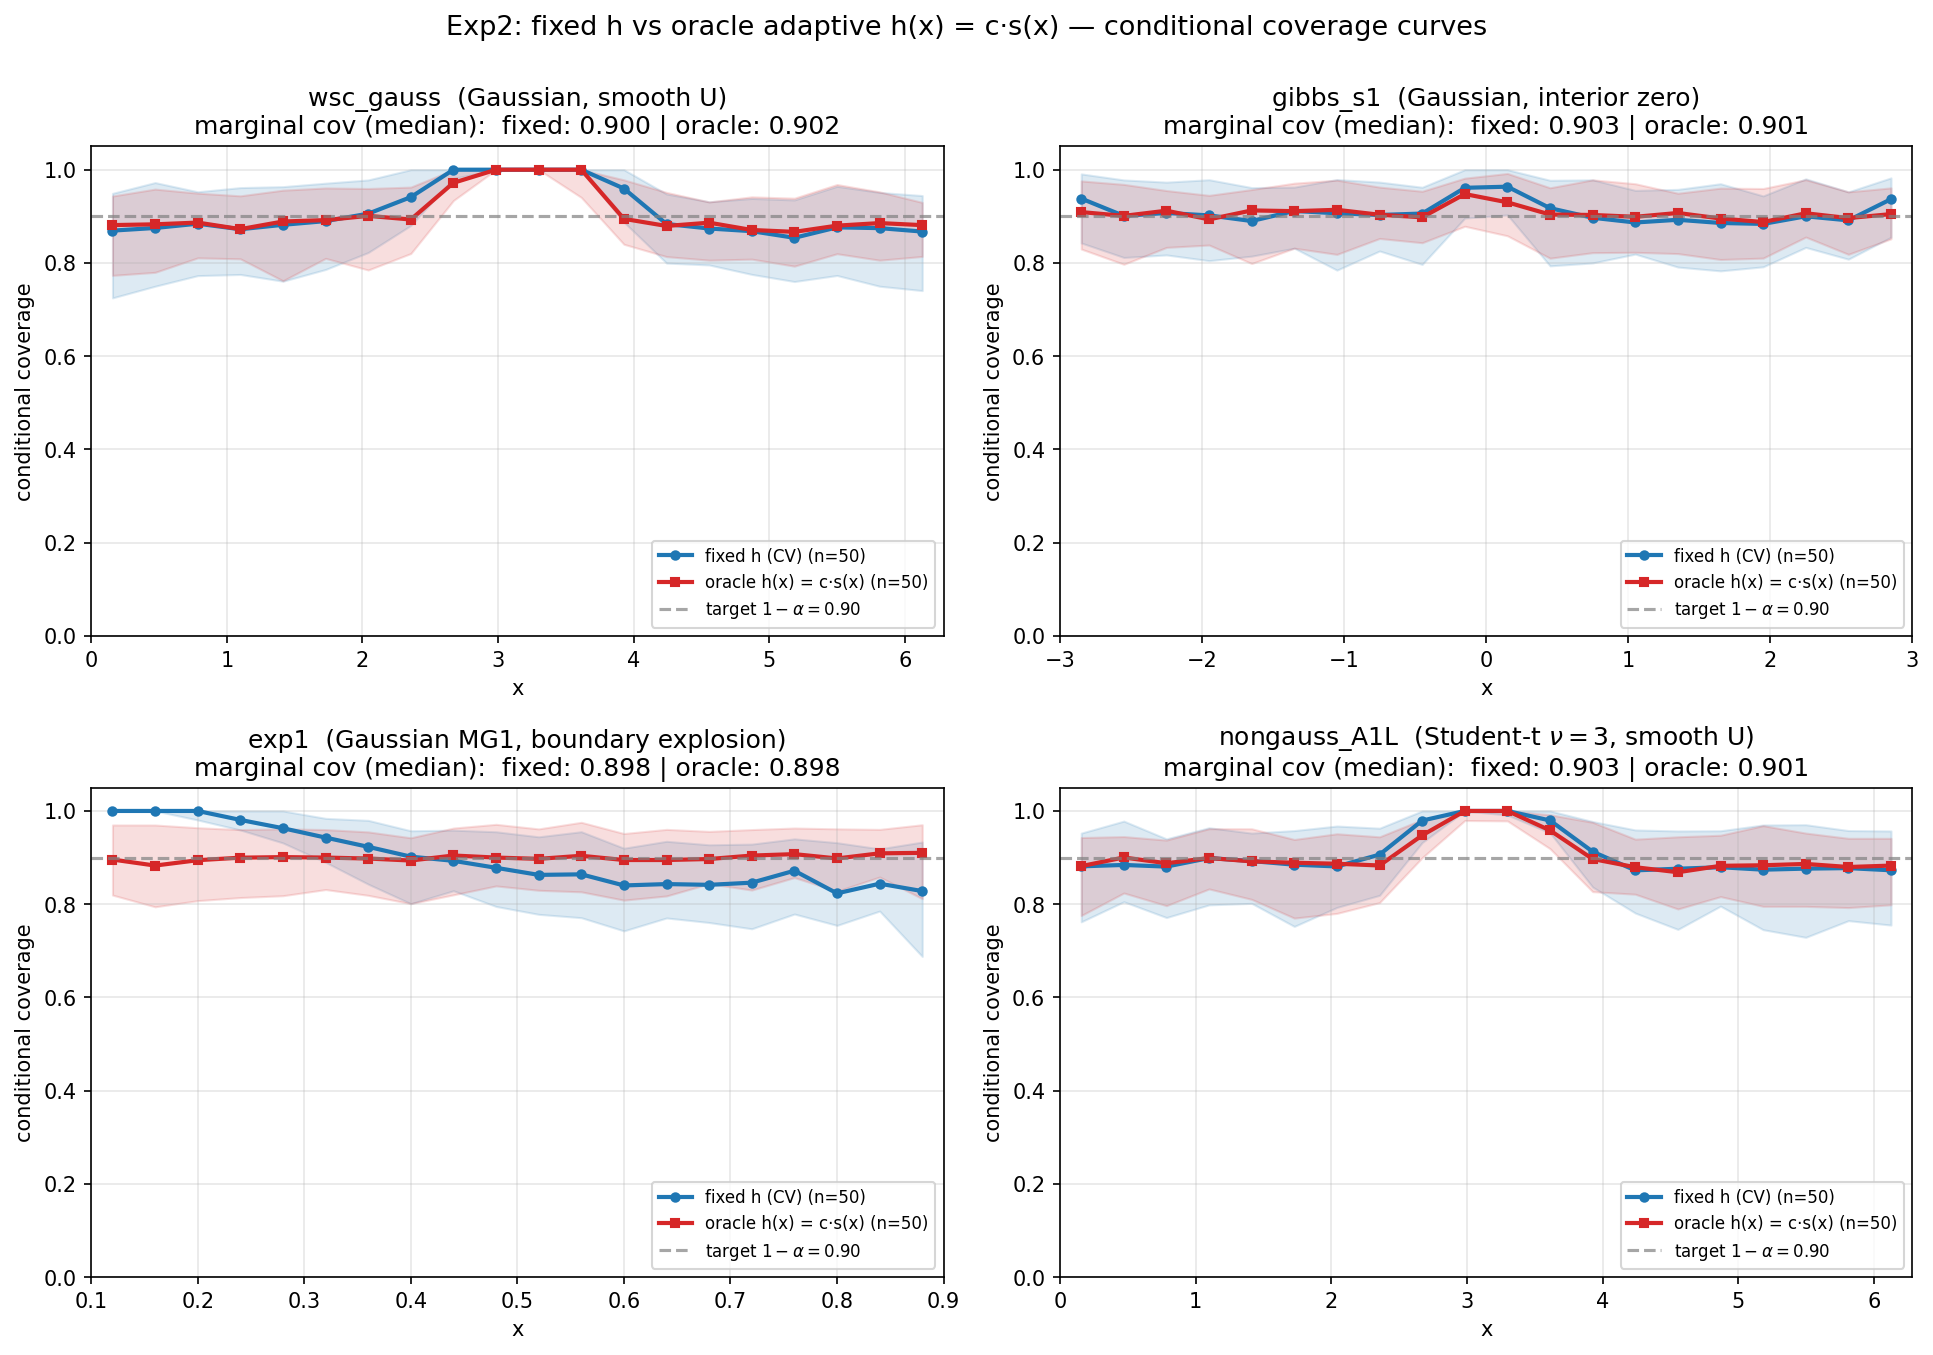
\includegraphics[width=0.86\linewidth]{exp2_oracle_vs_fixed_coverage.png}
\caption{Bin-wise coverage curves for fixed and oracle adaptive smoothing. Oracle adaptive smoothing flattens coverage across input bins while keeping marginal coverage near the conformal target.}
\label{fig:oracle-curves}
\end{figure}
}{}

\subsection{Choice of the multiplier \texorpdfstring{\(c\)}{c}}

The multiplier \(c\) controls the smoothing scale relative to the local response scale. A sweep on \texttt{nongauss\_A1L} shows that worst-bin coverage deviation improves from the fixed baseline \(0.136\) to \(0.105\) at \(c=1\), with little additional gain at \(c=2\). We therefore use \(c=1\) as the default in the plug-in experiments.

\begin{table}[t]
\centering
\caption{\(c\)-sweep on \texttt{nongauss\_A1L}. The fixed row is the scalar-bandwidth baseline.}
\label{tab:c-sweep}
\resizebox{\linewidth}{!}{%
% Exp3 c-sweep on nongauss_A1L. Target marginal coverage = 0.90.
% Cell format: median (sd) for binwise stats; mean (sd) for width and IS.
\begin{tabular}{lrrrrrr}
\toprule
arm & $c$ & marginal cov & worst-bin $|c-(1-\alpha)|$ & mean-bin $|c-(1-\alpha)|$ & mean width & mean IS \\
\midrule
fixed & --- & 0.903 (0.013) & 0.136 (0.041) & 0.056 (0.009) & 3.179 (0.275) & 5.549 (0.774) \\
c0.3 & 0.3 & 0.899 (0.013) & 0.115 (0.034) & 0.052 (0.008) & 3.129 (0.226) & 5.410 (0.758) \\
c0.5 & 0.5 & 0.901 (0.012) & 0.113 (0.028) & 0.050 (0.007) & 3.037 (0.178) & 5.341 (0.752) \\
c1 & 1 & 0.901 (0.012) & 0.105 (0.021) & 0.046 (0.007) & 2.988 (0.150) & 5.276 (0.744) \\
c2 & 2 & 0.900 (0.012) & 0.104 (0.020) & 0.042 (0.007) & 3.009 (0.153) & 5.251 (0.742) \\
\bottomrule
\end{tabular}

}
\end{table}

\fi

\section{Positioning Relative to Existing CP Methods}
\label{sec:positioning}

The proposed method does not make conformal validity depend on CKME itself. Split conformal validity is estimator-agnostic once calibration and target samples are exchangeable under the target law. CKME enters through the score-construction layer, where a better conditional CDF estimator and a better smoothing scale can improve interval efficiency and groupwise behavior. The target-aware formulation therefore separates two roles:
\[
  \begin{aligned}
  &\text{target-aware calibration specifies where validity holds,}\\
  &\text{scale-adaptive CKME improves the DCP score used for efficiency.}
  \end{aligned}
\]

Conformalized quantile regression adapts interval endpoints through estimated conditional quantiles \cite{romano2019}. Distribution regression versions of DCP estimate the conditional CDF through threshold-indexed regressions \cite{chernozhukov2021}. Localized and weighted conformal methods modify the calibration distribution or score weighting to improve local guarantees \cite{tibshirani2019,hore2025}. CKME-DCP is complementary: it estimates a single conditional distributional object and uses smooth test functions to evaluate CDFs. This representation creates a bandwidth parameter whose local scaling can be matched to the response scale.

This distinction also clarifies the role of adaptive design. Adaptive site selection changes where simulation data are collected. It is a data-acquisition layer and can improve estimator quality in high-uncertainty regions, but it is not the same contribution as scale-adaptive smoothing. The present paper keeps the theorem line focused on target validity and scale-adaptive scoring.

\section{Discussion}
\label{sec:discussion}

This paper separates the validity layer and the score-efficiency layer in CKME-DCP for stochastic simulation outputs. The validity layer is the split-conformal argument under a stated target joint law \(P^q_{XY}=q_XP_{Y\mid X}\). The score-efficiency layer is the CKME conditional CDF estimator and, in particular, the smooth-indicator bandwidth used to evaluate DCP scores.

The target formulation makes the coverage statement explicit. Global-domain coverage, region-of-interest coverage, fixed-target-set average coverage, and smoothed fixed-target local coverage are different claims because they integrate over different input laws. The finite-sample split-conformal guarantee applies cleanly in the matched target-calibration setting, while target mismatch requires reweighting or a separate calibration design.

The scale-adaptive bandwidth addresses a different problem. Under heteroscedasticity, fixed smoothing creates the standardized ratio \(h/s(x)\), so the same output-side bandwidth can represent different amounts of smoothing in low- and high-variance regions. Setting \(h(x)=c\widehat s(x)\) aligns the smoothed indicator with local response scale. The oracle analysis shows the mechanism.

\ifincludeexperiments
The present experiments focus on calibrated interval performance rather than raw CDF estimation alone. Raw CDF diagnostics are useful for mechanism checks, but the inferential targets are coverage, width, interval score, and groupwise stability after conformal calibration. The current numerical evidence supports the scale-adaptive smoothing claim under matched global target distributions. Region-of-interest targets and external conformal or simulation-UQ baselines are natural extensions, but they are not needed for the finite-sample validity statement or for isolating the bandwidth mechanism studied here.
\fi

\appendix

\section{Proofs}
\label{app:proofs}

\subsection{Proof of Proposition~\ref{prop:target-validity}}

Condition on the training data and on the fitted estimator \(\widehat F\). Under the stated exchangeability condition, the calibration scores
\[
  S_i^{\mathrm{cal}}=S_{\widehat F}(X_i^{\mathrm{cal}},Y_i^{\mathrm{cal}}),
  \qquad i=1,\ldots,n_{\mathrm{cal}},
\]
and the target score
\[
  S_\star=S_{\widehat F}(X_\star,Y_\star)
\]
are exchangeable. Let
\[
  k=\left\lceil (n_{\mathrm{cal}}+1)(1-\alpha)\right\rceil .
\]
If \(k\le n_{\mathrm{cal}}\), \(\widehat q_{1-\alpha}\) is the \(k\)-th order statistic of the calibration scores; if \(k=n_{\mathrm{cal}}+1\), the usual convention is \(\widehat q_{1-\alpha}=+\infty\), in which case the claim is trivial. For \(k\le n_{\mathrm{cal}}\), the rank of \(S_\star\) among the \(n_{\mathrm{cal}}+1\) exchangeable scores is uniform up to ties, and the conservative tie convention gives
\[
  \Pp\{S_\star\le \widehat q_{1-\alpha}\mid \Dcal_{\mathrm{tr}},\widehat F\}
  \ge
  \frac{k}{n_{\mathrm{cal}}+1}
  \ge
  1-\alpha .
\]
Since \(Y_\star\in\widehat C(X_\star)\) is exactly the event \(S_\star\le\widehat q_{1-\alpha}\), taking expectation over the training data proves
\[
  \Pp_{(X,Y)\sim P^q_{XY}}\{Y\in\widehat C(X)\}\ge 1-\alpha .
\]

\subsection{Proof of Proposition~\ref{prop:error-transfer}}

Let \(A(u)=|u-1/2|\). This map is one-Lipschitz. On the event in Assumption~\ref{ass:uniform},
\[
\begin{aligned}
  \abs{S_{\widehat F}(x,y)-S^\circ(x,y)}
  &=
  \abs{A(\widehat F(y\mid x))-A(F^\circ(y\mid x))}  \\
  &\le
  \abs{\widehat F(y\mid x)-F^\circ(y\mid x)}
  \le \epsilon_n
\end{aligned}
\]
uniformly over \(x\in\Xcal\) and \(y\in\Tcal\). This proves the score perturbation bound.

For the threshold statement, define the oracle calibration scores
\[
  S_i^\circ=S^\circ(X_i^{\mathrm{cal}},Y_i^{\mathrm{cal}}),
  \qquad i=1,\ldots,n_{\mathrm{cal}},
\]
and let \(q_{n,1-\alpha}^\circ\) be their \(k\)-th order statistic, with the same \(k=\lceil(n_{\mathrm{cal}}+1)(1-\alpha)\rceil\). The uniform score perturbation bound implies
\[
  \max_{1\le i\le n_{\mathrm{cal}}}
  \abs{\widehat S_i-S_i^\circ}
  \le \epsilon_n.
\]
Order statistics are one-Lipschitz with respect to the sup-norm perturbation of the sample, hence
\[
  \abs{\widehat q_{1-\alpha}-q_{n,1-\alpha}^\circ}
  \le \epsilon_n.
\]
By Assumption~\ref{ass:score}, the oracle score distribution is regular at \(q^\circ_{1-\alpha}\). Standard empirical-quantile theory gives
\[
  \abs{q_{n,1-\alpha}^\circ-q^\circ_{1-\alpha}}
  =
  \Op(n_{\mathrm{cal}}^{-1/2}).
\]
Combining the two displays yields
\[
  \abs{\widehat q_{1-\alpha}-q^\circ_{1-\alpha}}
  =
  \Op(\epsilon_n+n_{\mathrm{cal}}^{-1/2}).
\]

\subsection{Proof of Theorem~\ref{thm:homogeneity}}

Under \(Y=m(x)+s(x)\varepsilon\) and \(h(x)=c s(x)\),
\[
  F_c^\circ(y\mid x)=
  H_c\!\left(\frac{y-m(x)}{s(x)}\right).
\]
Evaluating at \(Y=m(x)+s(x)\varepsilon\) gives
\[
  F_c^\circ(Y\mid X=x)
  =
  H_c(\varepsilon).
\]
Because \(\varepsilon\perp X\), the conditional distribution of \(H_c(\varepsilon)\) given \(X=x\) is the same for all \(x\). Applying any measurable transform \(A\) preserves equality in distribution, so
\[
  S_c^\circ(X,Y)\mid X=x
  =
  A(F_c^\circ(Y\mid X=x))
  \overset{d}{=}
  A(H_c(\varepsilon)).
\]

\subsection{Proof of Proposition~\ref{prop:plugin-oracle}}

Write
\[
  z_x(t)=\frac{t-m(x)}{s(x)}.
\]
Under the location-scale model,
\[
  \frac{t-Y}{c\widehat s(x)}
  =
  \frac{z_x(t)-\varepsilon}{c}\frac{s(x)}{\widehat s(x)},
  \qquad
  \frac{t-Y}{c s(x)}
  =
  \frac{z_x(t)-\varepsilon}{c}.
\]
On the event \(\Delta_n<1/2\),
\[
  \sup_{x\in\Xcal}
  \abs{\frac{s(x)}{\widehat s(x)}-1}
  =
  \sup_{x\in\Xcal}
  \abs{\frac{1}{\widehat s(x)/s(x)}-1}
  \le
  2\Delta_n .
\]
Using the Lipschitz property of \(\Psi\), for every \(x,t\),
\[
\begin{aligned}
  &\abs{F_{\widehat h}^{\circ}(t\mid x)-F_c^\circ(t\mid x)} \\
  &\quad\le
  \E\left[
  L_\Psi
  \abs{\frac{z_x(t)-\varepsilon}{c}}
  \abs{\frac{s(x)}{\widehat s(x)}-1}
  \middle|X=x
  \right]  \\
  &\quad\le
  \frac{2L_\Psi}{c}\Delta_n
  \E\left[
  \abs{z_x(t)-\varepsilon}
  \middle|X=x
  \right].
\end{aligned}
\]
Taking the supremum over \(x\in\Xcal\) and \(t\in\Tcal\), and applying Assumption~\ref{ass:std-moment}, gives
\[
  \sup_{x,t}
  \abs{F_{\widehat h}^{\circ}(t\mid x)-F_c^\circ(t\mid x)}
  \le
  \frac{2L_\Psi M_{\Tcal}}{c}\Delta_n
\]
with probability tending to one. Assumption~\ref{ass:scale} gives the result.

\subsection{Proof of Proposition~\ref{prop:ckme-cdf}}

For every \(x,t\),
\[
  \abs{\widehat F_{h(\cdot)}(t\mid x)-F_{h(\cdot)}^\circ(t\mid x)}
  =
  \abs{\inner{g_{t,h(x)}}{\widehat\mu_{Y\mid x}-\mu_{Y\mid x}}_{\Hcal_Y}}
  \le
  \norm{g_{t,h(x)}}_{\Hcal_Y}
  \norm{\widehat\mu_{Y\mid x}-\mu_{Y\mid x}}_{\Hcal_Y}.
\]
Taking suprema and applying Assumptions~\ref{ass:ckme}--\ref{ass:g} gives the result.

\subsection{Proof of Theorem~\ref{thm:group}}

Let
\[
  \widehat S(x,y)=S_{\widehat F}(x,y),
  \qquad
  S_c^\circ(x,y)=\abs{F_c^\circ(y\mid x)-1/2}.
\]
By Proposition~\ref{prop:ckme-cdf} and Proposition~\ref{prop:error-transfer}, there exists a sequence \(r_n=\op(1)\) such that, with probability tending to one,
\[
  \sup_{x,y}\abs{\widehat S(x,y)-S_c^\circ(x,y)}\le r_n,
  \qquad
  \abs{\widehat q_{1-\alpha}-q^\circ_{1-\alpha}}\le r_n.
\]
On this event, for any group \(\Gcal_k\),
\[
  \{S_c^\circ(X,Y)\le q^\circ_{1-\alpha}-2r_n\}
  \subseteq
  \{\widehat S(X,Y)\le \widehat q_{1-\alpha}\}
  \subseteq
  \{S_c^\circ(X,Y)\le q^\circ_{1-\alpha}+2r_n\}.
\]
Therefore,
\[
\begin{aligned}
  &\abs{
  \Pp\{\widehat S(X,Y)\le\widehat q_{1-\alpha}\mid X\in\Gcal_k\}
  -
  \Pp\{S_c^\circ(X,Y)\le q^\circ_{1-\alpha}\mid X\in\Gcal_k\}
  }  \\
  &\quad\le
  \sup_{\abs{u-q^\circ_{1-\alpha}}\le 2r_n}
  \abs{G_k(u)-G_k(q^\circ_{1-\alpha})},
\end{aligned}
\]
where \(G_k\) is the groupwise oracle score CDF in Assumption~\ref{ass:group}. By the uniform Lipschitz condition, the right-hand side is \(O(r_n)=\op(1)\), uniformly over the fixed finite set of groups.

It remains to identify the oracle group coverage level. Theorem~\ref{thm:homogeneity} implies that the conditional distribution of \(S_c^\circ(X,Y)\) given \(X=x\) does not depend on \(x\). Hence every group has the same oracle score distribution as the marginal target distribution:
\[
  \Pp\{S_c^\circ(X,Y)\le u\mid X\in\Gcal_k\}
  =
  \Pp\{S_c^\circ(X,Y)\le u\}.
\]
At the continuity point \(q^\circ_{1-\alpha}\), this probability equals \(1-\alpha\). Thus
\[
  \max_{1\le k\le K}
  \abs{
  \Pp\{Y\in\widehat C(X)\mid X\in\Gcal_k\}
  -(1-\alpha)
  }
  \to 0
\]
in probability.

\subsection{Proof of Corollary~\ref{cor:plugin-group}}

Let \(F_{\widehat h}^{\circ}\) denote the plug-in smoothed oracle CDF and let \(F_c^\circ\) denote the oracle adaptive smoothed CDF. By the assumed uniform CKME consistency for \(F_{\widehat h}^{\circ}\),
\[
  \sup_{x,t}
  \abs{\widehat F_{h(\cdot)}(t\mid x)-F_{\widehat h}^{\circ}(t\mid x)}
  =
  \op(1).
\]
By Proposition~\ref{prop:plugin-oracle},
\[
  \sup_{x,t}
  \abs{F_{\widehat h}^{\circ}(t\mid x)-F_c^\circ(t\mid x)}
  =
  \op(1).
\]
The triangle inequality gives
\[
  \sup_{x,t}
  \abs{\widehat F_{h(\cdot)}(t\mid x)-F_c^\circ(t\mid x)}
  =
  \op(1).
\]
Thus Assumption~\ref{ass:uniform} holds with \(F^\circ=F_c^\circ\), up to replacing \(\epsilon_n\) by the sum of the CKME and plug-in scale errors. The proof of Theorem~\ref{thm:group} then applies verbatim.

\begin{thebibliography}{99}

\bibitem{angelopoulos2023}
A.~N. Angelopoulos and S.~Bates.
\newblock Conformal prediction: A gentle introduction.
\newblock \emph{Foundations and Trends in Machine Learning}, 16(4):494--591, 2023.

\bibitem{ankenman2010}
B.~Ankenman, B.~L. Nelson, and J.~Staum.
\newblock Stochastic kriging for simulation metamodeling.
\newblock \emph{Operations Research}, 58(2):371--382, 2010.

\bibitem{binois2018}
M.~Binois, R.~B. Gramacy, and M.~Ludkovski.
\newblock Practical heteroscedastic Gaussian process modeling for large simulation experiments.
\newblock \emph{Journal of Computational and Graphical Statistics}, 27(4):808--821, 2018.

\bibitem{chernozhukov2021}
V.~Chernozhukov, K.~Wuthrich, and Y.~Zhu.
\newblock Distributional conformal prediction.
\newblock \emph{Proceedings of the National Academy of Sciences}, 118(48):e2107794118, 2021.

\bibitem{hore2025}
R.~Hore and R.~F. Barber.
\newblock Localized conformal prediction.
\newblock 2025.

\bibitem{lei2018}
J.~Lei, M.~G'Sell, A.~Rinaldo, R.~J. Tibshirani, and L.~Wasserman.
\newblock Distribution-free predictive inference for regression.
\newblock \emph{Journal of the American Statistical Association}, 113(523):1094--1111, 2018.

\bibitem{muandet2017}
K.~Muandet, K.~Fukumizu, B.~Sriperumbudur, and B.~Scholkopf.
\newblock Kernel mean embedding of distributions: A review and beyond.
\newblock \emph{Foundations and Trends in Machine Learning}, 10(1--2):1--141, 2017.

\bibitem{romano2019}
Y.~Romano, E.~Patterson, and E.~J. Candes.
\newblock Conformalized quantile regression.
\newblock \emph{Advances in Neural Information Processing Systems}, 2019.

\bibitem{sacks1989}
J.~Sacks, W.~J. Welch, T.~J. Mitchell, and H.~P. Wynn.
\newblock Design and analysis of computer experiments.
\newblock \emph{Statistical Science}, 4(4):409--423, 1989.

\bibitem{shafer2008}
G.~Shafer and V.~Vovk.
\newblock A tutorial on conformal prediction.
\newblock \emph{Journal of Machine Learning Research}, 9:371--421, 2008.

\bibitem{song2013}
L.~Song, K.~Fukumizu, and A.~Gretton.
\newblock Kernel embeddings of conditional distributions.
\newblock \emph{IEEE Signal Processing Magazine}, 30(4):98--111, 2013.

\bibitem{tibshirani2019}
R.~J. Tibshirani, R.~Foygel Barber, E.~Candes, and A.~Ramdas.
\newblock Conformal prediction under covariate shift.
\newblock \emph{Advances in Neural Information Processing Systems}, 2019.

\bibitem{vovk2005}
V.~Vovk, A.~Gammerman, and G.~Shafer.
\newblock \emph{Algorithmic Learning in a Random World}.
\newblock Springer, 2005.

\end{thebibliography}

\end{document}
